% Options for packages loaded elsewhere
\PassOptionsToPackage{unicode}{hyperref}
\PassOptionsToPackage{hyphens}{url}
\PassOptionsToPackage{dvipsnames,svgnames,x11names}{xcolor}
%
\documentclass[
  10pt,
  a4paper,
  a4paper]{article}

\usepackage{amsmath,amssymb}
\usepackage{iftex}
\ifPDFTeX
  \usepackage[T1]{fontenc}
  \usepackage[utf8]{inputenc}
  \usepackage{textcomp} % provide euro and other symbols
\else % if luatex or xetex
  \usepackage{unicode-math}
  \defaultfontfeatures{Scale=MatchLowercase}
  \defaultfontfeatures[\rmfamily]{Ligatures=TeX,Scale=1}
\fi
\usepackage{lmodern}
\ifPDFTeX\else  
    % xetex/luatex font selection
  \setmainfont[]{Latin Modern Roman}
  \setsansfont[]{Latin Modern Roman}
\fi
% Use upquote if available, for straight quotes in verbatim environments
\IfFileExists{upquote.sty}{\usepackage{upquote}}{}
\IfFileExists{microtype.sty}{% use microtype if available
  \usepackage[]{microtype}
  \UseMicrotypeSet[protrusion]{basicmath} % disable protrusion for tt fonts
}{}
\makeatletter
\@ifundefined{KOMAClassName}{% if non-KOMA class
  \IfFileExists{parskip.sty}{%
    \usepackage{parskip}
  }{% else
    \setlength{\parindent}{0pt}
    \setlength{\parskip}{6pt plus 2pt minus 1pt}}
}{% if KOMA class
  \KOMAoptions{parskip=half}}
\makeatother
\usepackage{xcolor}
\usepackage[top=25mm,left=35mm,right=20mm,bottom=24mm]{geometry}
\setlength{\emergencystretch}{3em} % prevent overfull lines
\setcounter{secnumdepth}{5}
% Make \paragraph and \subparagraph free-standing
\ifx\paragraph\undefined\else
  \let\oldparagraph\paragraph
  \renewcommand{\paragraph}[1]{\oldparagraph{#1}\mbox{}}
\fi
\ifx\subparagraph\undefined\else
  \let\oldsubparagraph\subparagraph
  \renewcommand{\subparagraph}[1]{\oldsubparagraph{#1}\mbox{}}
\fi


\providecommand{\tightlist}{%
  \setlength{\itemsep}{0pt}\setlength{\parskip}{0pt}}\usepackage{longtable,booktabs,array}
\usepackage{calc} % for calculating minipage widths
% Correct order of tables after \paragraph or \subparagraph
\usepackage{etoolbox}
\makeatletter
\patchcmd\longtable{\par}{\if@noskipsec\mbox{}\fi\par}{}{}
\makeatother
% Allow footnotes in longtable head/foot
\IfFileExists{footnotehyper.sty}{\usepackage{footnotehyper}}{\usepackage{footnote}}
\makesavenoteenv{longtable}
\usepackage{graphicx}
\makeatletter
\def\maxwidth{\ifdim\Gin@nat@width>\linewidth\linewidth\else\Gin@nat@width\fi}
\def\maxheight{\ifdim\Gin@nat@height>\textheight\textheight\else\Gin@nat@height\fi}
\makeatother
% Scale images if necessary, so that they will not overflow the page
% margins by default, and it is still possible to overwrite the defaults
% using explicit options in \includegraphics[width, height, ...]{}
\setkeys{Gin}{width=\maxwidth,height=\maxheight,keepaspectratio}
% Set default figure placement to htbp
\makeatletter
\def\fps@figure{htbp}
\makeatother

\makeatletter
\makeatother
\makeatletter
\makeatother
\makeatletter
\@ifpackageloaded{caption}{}{\usepackage{caption}}
\AtBeginDocument{%
\ifdefined\contentsname
  \renewcommand*\contentsname{Table of contents}
\else
  \newcommand\contentsname{Table of contents}
\fi
\ifdefined\listfigurename
  \renewcommand*\listfigurename{List of Figures}
\else
  \newcommand\listfigurename{List of Figures}
\fi
\ifdefined\listtablename
  \renewcommand*\listtablename{List of Tables}
\else
  \newcommand\listtablename{List of Tables}
\fi
\ifdefined\figurename
  \renewcommand*\figurename{Figure}
\else
  \newcommand\figurename{Figure}
\fi
\ifdefined\tablename
  \renewcommand*\tablename{Table}
\else
  \newcommand\tablename{Table}
\fi
}
\@ifpackageloaded{float}{}{\usepackage{float}}
\floatstyle{ruled}
\@ifundefined{c@chapter}{\newfloat{codelisting}{h}{lop}}{\newfloat{codelisting}{h}{lop}[chapter]}
\floatname{codelisting}{Listing}
\newcommand*\listoflistings{\listof{codelisting}{List of Listings}}
\makeatother
\makeatletter
\@ifpackageloaded{caption}{}{\usepackage{caption}}
\@ifpackageloaded{subcaption}{}{\usepackage{subcaption}}
\makeatother
\makeatletter
\@ifpackageloaded{tcolorbox}{}{\usepackage[skins,breakable]{tcolorbox}}
\makeatother
\makeatletter
\@ifundefined{shadecolor}{\definecolor{shadecolor}{HTML}{31BAE9}}
\makeatother
\makeatletter
\@ifundefined{codebgcolor}{\definecolor{codebgcolor}{HTML}{aadce3}}
\makeatother
\makeatletter
\makeatother
\ifLuaTeX
  \usepackage{selnolig}  % disable illegal ligatures
\fi
\IfFileExists{bookmark.sty}{\usepackage{bookmark}}{\usepackage{hyperref}}
\IfFileExists{xurl.sty}{\usepackage{xurl}}{} % add URL line breaks if available
\urlstyle{same} % disable monospaced font for URLs
\hypersetup{
  pdftitle={Advance HPC - Project},
  pdfauthor={Hoang Manh Truong},
  colorlinks=true,
  linkcolor={blue},
  filecolor={Maroon},
  citecolor={Blue},
  urlcolor={Blue},
  pdfcreator={LaTeX via pandoc}}

\title{Advance HPC - Project}
\author{Hoang Manh Truong}
\date{2023-11-05}

\begin{document}
\maketitle
\ifdefined\Shaded\renewenvironment{Shaded}{\begin{tcolorbox}[breakable, boxrule=0pt, enhanced, sharp corners, colback={codebgcolor}, borderline west={3pt}{0pt}{shadecolor}, frame hidden]}{\end{tcolorbox}}\fi

\hypertarget{versions}{%
\section{Versions}\label{versions}}

\begin{enumerate}
\def\labelenumi{\arabic{enumi}.}
\tightlist
\item
  CPU (using numpy)
\item
  CPU (using pure python)
\item
  GPU (non-shared memory)
\item
  GPU (shared memory)
\end{enumerate}

\hypertarget{steps}{%
\section{Steps}\label{steps}}

Given parameter \(\omega\) as window size

\begin{enumerate}
\def\labelenumi{\arabic{enumi}.}
\tightlist
\item
  Convert RGB to HSV (SCATTER)
\item
  For each pixel \(\Phi(i, j)\)
\item
  Define use 4 windows \(W^k\), \(k \in [1..4]\) of size
  \((\omega + 1) \times (\omega + 1)\)

  \begin{itemize}
  \tightlist
  \item
    \(W^1_x \in [i - \omega, i]\), \(W^1_y \in [j - \omega, j]\)
  \item
    \(W^2_x \in [i, i + \omega]\), \(W^2_y \in [j - \omega, j]\)
  \item
    \(W^3_x \in [i - \omega, i]\), \(W^3_y \in [j, j + \omega]\)
  \item
    \(W^4_x \in [i, i + \omega]\), \(W^4_y \in [j, j + \omega]\)
  \end{itemize}
\item
  Find \(W_l\), \(l \in [1..4]\) having the lowest standard deviation of
  brightness.

  \begin{itemize}
  \tightlist
  \item
    Use \(V\) in HSV color space to calculate SD.
  \end{itemize}
\item
  Assign mean \((R, G, B)\) value of this window
  \(\left| W_l \right|_{\text{RGB}}\) as new color (REDUCE, MAP)
\end{enumerate}

\[\Phi(i, j)_{\text{RGB}} = \left| W_l \right|_{\text{RGB}}\]

\hypertarget{results}{%
\section{Results}\label{results}}

\hypertarget{cpu-methods}{%
\subsection{CPU methods}\label{cpu-methods}}

For this project, two approaches are used that utilize CPU:

\begin{itemize}
\tightlist
\item
  Using numpy for the computation
\item
  Using pure python for the computation
\end{itemize}

The results are shown in the following table:

\begin{longtable}[]{@{}llll@{}}
\toprule\noalign{}
& type & time & window\_size \\
\midrule\noalign{}
\endhead
\bottomrule\noalign{}
\endlastfoot
0 & cpu\_numpy & 68.953223 & 3 \\
1 & cpu\_numpy & 71.472559 & 5 \\
2 & cpu\_numpy & 67.938109 & 7 \\
3 & cpu\_numpy & 68.209134 & 9 \\
4 & cpu\_numpy & 66.368311 & 11 \\
5 & cpu\_numpy & 69.186078 & 13 \\
6 & cpu\_numpy & 73.795276 & 15 \\
7 & cpu\_numpy & 77.442831 & 17 \\
8 & cpu\_numpy & 81.551760 & 19 \\
9 & cpu\_pure\_python & 323.052644 & 3 \\
10 & cpu\_pure\_python & 415.845123 & 5 \\
11 & cpu\_pure\_python & 581.276988 & 7 \\
12 & cpu\_pure\_python & 689.937136 & 9 \\
\end{longtable}

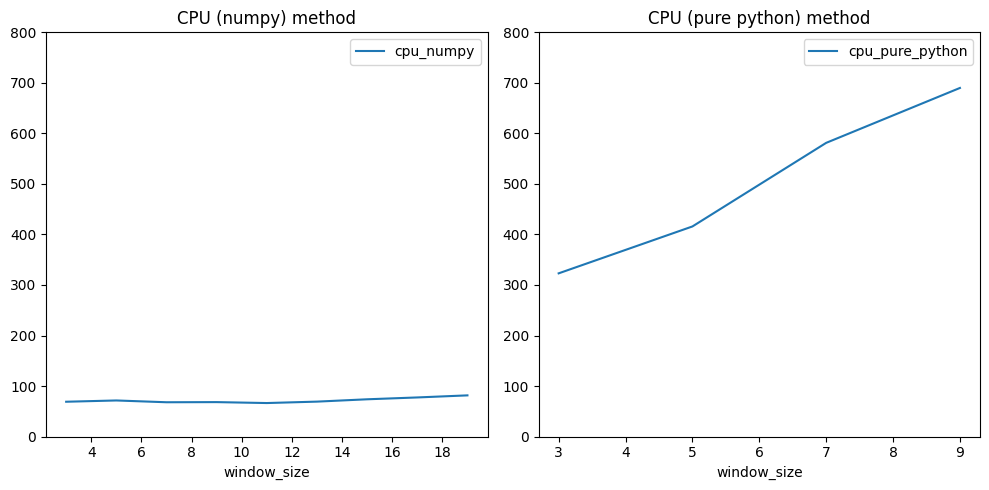
\includegraphics{Report.10.kuwahara_files/figure-pdf/cell-5-output-1.png}

As shown in the figure and table:

\begin{itemize}
\item
  \textbf{The CPU numpy approach} on average takes about 70 seconds to
  run. This is much faster than the pure python approach (which takes
  from 300 to 700 seconds), and has an approximately constant runtime
  for different window sizes. This is probably due to the nature of
  numpy, which is optimized for vectorized computation.
\item
  \textbf{The pure Python approach} is much slower than the numpy
  approach, and have a runtime that increases with the window size. This
  is due to the use of nested loop, meaning that the time complexity
  scales with the window size and the sizes of the image.
\end{itemize}

\hypertarget{gpu-methods}{%
\subsection{GPU methods}\label{gpu-methods}}

For the GPU approach, one method are used:

\begin{itemize}
\tightlist
\item
  \textbf{Using GPU without shared memory}: Result included.
\item
  \textbf{Using GPU with shared memory}: The code is included, however
  it is not working properly and as such the result is omitted.
\end{itemize}

Each method is also run with different block sizes: \emph{(2,2), (4,4),
(8,8)}. Moreover, the results also exclude the time for initializing the
GPU, which is done only once, so that the results are more accurate and
not biased by the initialization time.

The results are shown in the following table:

\begin{longtable}[]{@{}lllll@{}}
\toprule\noalign{}
& type & time & window\_size & block\_size \\
\midrule\noalign{}
\endhead
\bottomrule\noalign{}
\endlastfoot
13 & gpu\_non\_shared & 0.078021 & 3 & (2, 2) \\
14 & gpu\_non\_shared & 0.141573 & 5 & (2, 2) \\
15 & gpu\_non\_shared & 0.229896 & 7 & (2, 2) \\
16 & gpu\_non\_shared & 0.360766 & 9 & (2, 2) \\
17 & gpu\_non\_shared & 0.019103 & 3 & (4, 4) \\
18 & gpu\_non\_shared & 0.036170 & 5 & (4, 4) \\
19 & gpu\_non\_shared & 0.059818 & 7 & (4, 4) \\
20 & gpu\_non\_shared & 0.093136 & 9 & (4, 4) \\
21 & gpu\_non\_shared & 0.010099 & 3 & (8, 8) \\
22 & gpu\_non\_shared & 0.019615 & 5 & (8, 8) \\
23 & gpu\_non\_shared & 0.031119 & 7 & (8, 8) \\
24 & gpu\_non\_shared & 0.047993 & 9 & (8, 8) \\
\end{longtable}

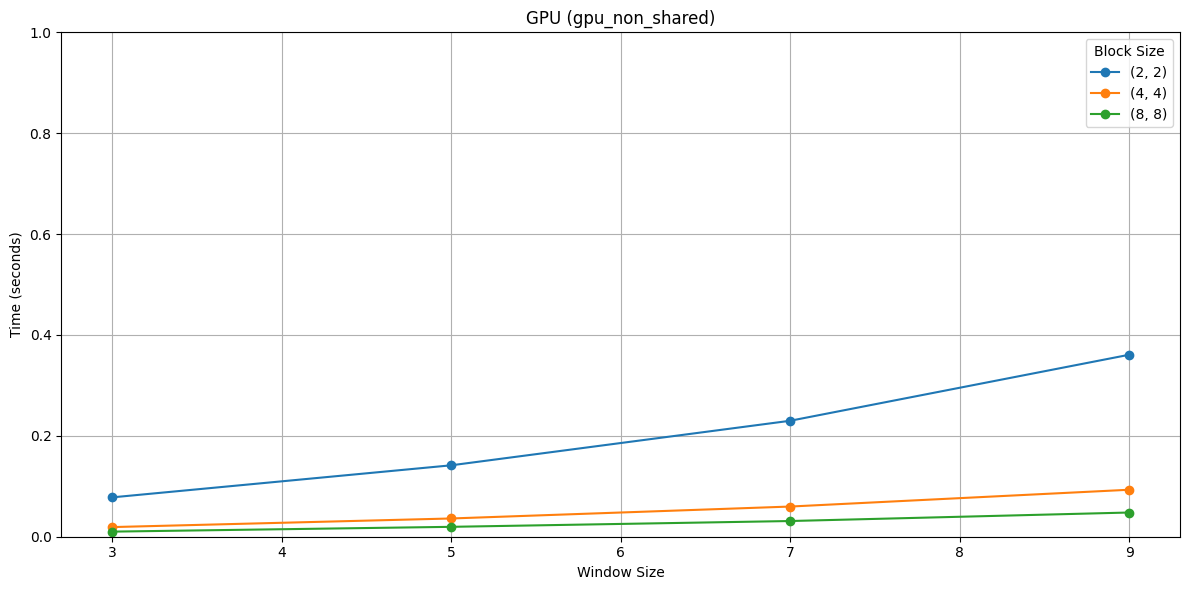
\includegraphics{Report.10.kuwahara_files/figure-pdf/cell-7-output-1.png}

As shown in the table and figure above, the runtime across different
block sizes increases with the window sizes. Moreover, the runtime
becomes smaller as the block size increases.



\end{document}
